Mediante la siguiente ilustración se observa el punto rojo en el espacio tridimensional con coordenadas esféricas ${\left(\rho,\theta,\varphi\right)}$, que proyecta un plano perpendicular al plano ${\left(x,y\right)}$, en dicho espacio se forman ${2}$ triángulos rectángulos. Es importante señalar que la variable ${r}$ es una coordenada polar que ayuda en la formación del triángulo rectángulo y su relación con las coordenadas ${\left(x,y\right)}$. Por ello, para el ángulo interno ${\varphi}$ se calcularán sus funciones trigonométricas.

\begin{figure}[H]
  \centering
  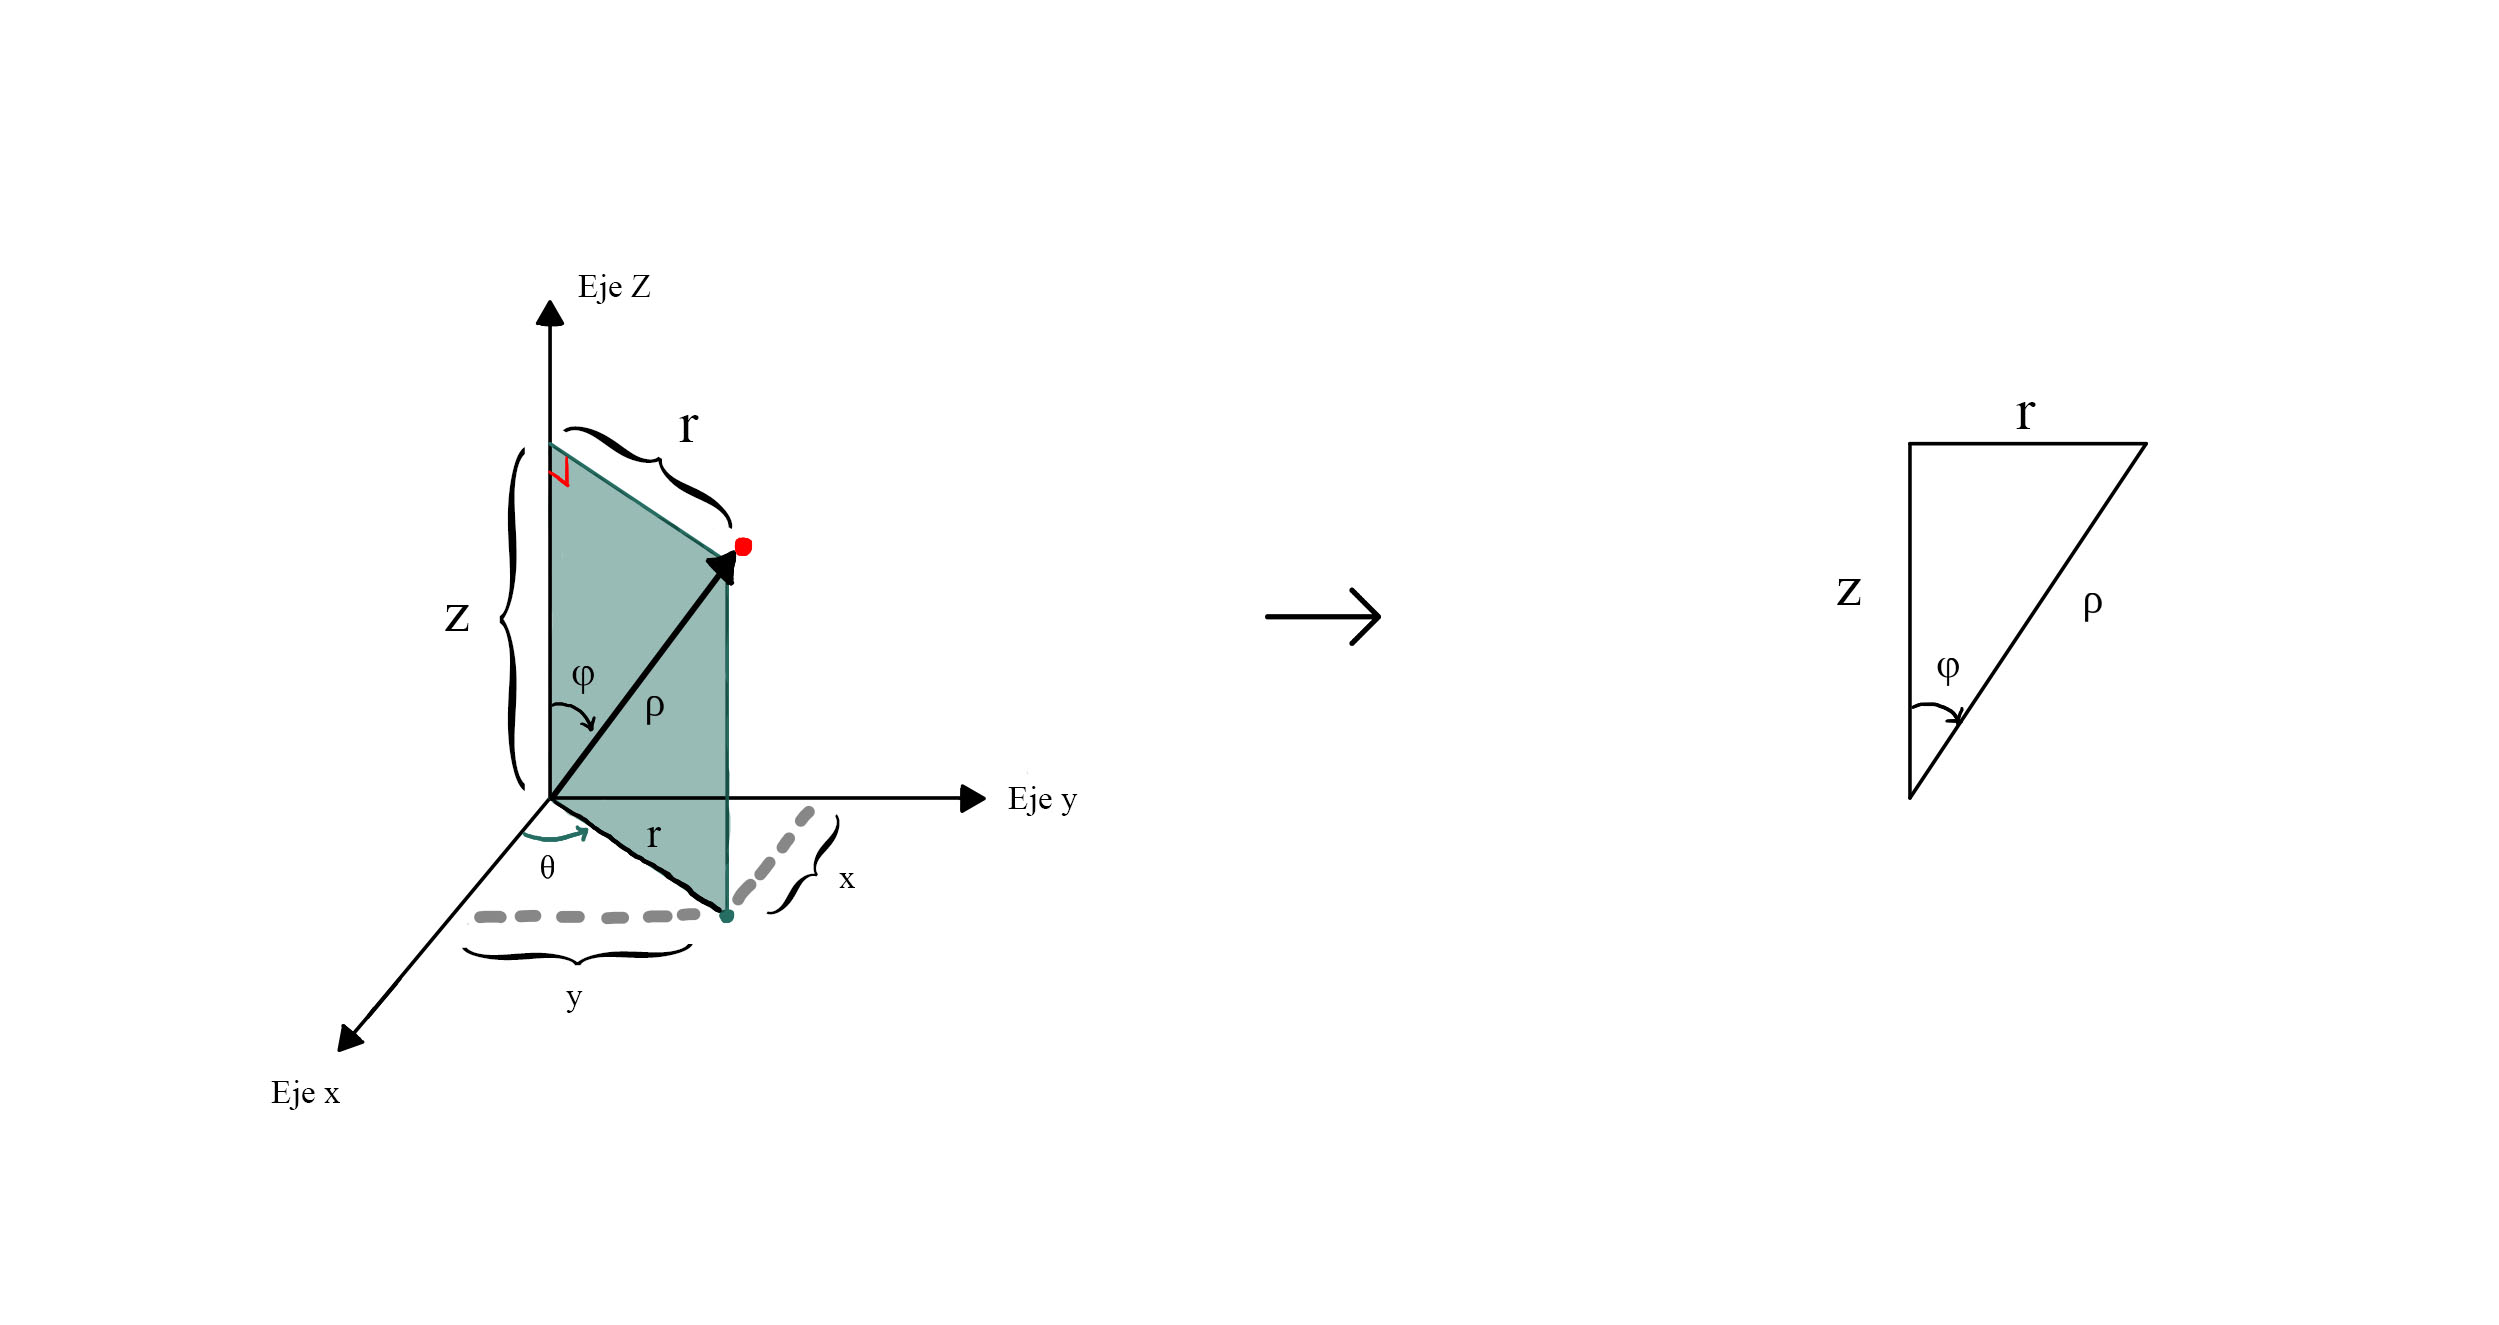
\includegraphics[width=11.17cm, height=5.67cm]{img/graph/coord_esf_2_rect_1.jpg}
  \caption{Triángulo rectángulo de un plano tridimensional.}
  \label{relacion_de_coordenadas}
\end{figure}

Entonces:
\begin{eqnarray*}
  \cos \varphi = \frac{\text{cateto adyacente}}{\text{hipotenusa}} = \frac{z}{\rho} \rightarrow z = \rho \cos \varphi\\\\
  \sin \varphi = \frac{\text{cateto opuesto}}{\text{hipotenusa}} = \frac{r}{\rho} \rightarrow r = \rho \sin \varphi
\end{eqnarray*}

\vspace{4mm}
Pero por la relación que se estableció con las coordenadas rectangulares y polares, entonces:

\begin{eqnarray*}
  x = r \cos \theta \rightarrow x = \rho \sin \varphi \cos \theta = \rho \cos \theta \sin \varphi\\\\
  y = r \sin \theta \rightarrow y = \rho \sin \varphi \sin \theta = \rho \sin \theta \sin \varphi
\end{eqnarray*}

\vspace{4mm}
Ahora, cuando se tienen coordenadas esféricas con el uso de dichas ecuaciones, se podrá determinar su equivalencia en coordenadas ${\left(x,y,z\right)}$.